%% ----------------------------------------------------------------
%% Project.tex
%% ----------------------------------------------------------------
\documentclass[openany]{ecsproject}     % Use the Project Style
\graphicspath{{images/}}   % Location of your graphics files
%\DeclareGraphicsExtensions{.png, .jpg, .eps}
\usepackage{pdfpages,listings,color,array}
\usepackage[titletoc]{appendix}
\usepackage[square,numbers]{natbib}            % Use Natbib style for the refs.
\hypersetup{colorlinks=true}   % Set to false for black/white printing
\input{Definitions}            % Include your abbreviations
%\bibliographystyle{ecs}

\bibliographystyle{ieeetr}
\renewcommand{\bibname}{References}
%% ----------------------------------------------------------------
\begin{document}
\frontmatter
\title      {Energy Efficient Object Detection and Tracking through Adaptive Operation on Heterogeneous Multi-core Systems}
\authors    {\texorpdfstring
             {\href{mailto:yz39g13@soton.ac.uk}{Yubo Zhi}}
             {Yubo Zhi}
            }
\addresses  {\groupname\\\deptname\\\univname}
\date       {\today}
\subject    {}
\keywords   {}
\supervisor {\texorpdfstring
             {\href{mailto:gvm@ecs.soton.ac.uk}{Dr Geoff Merrett}}
             {Dr Geoff Merrett}
	    }
\examiner   {\texorpdfstring
             {\href{mailto:dan@ecs.soton.ac.uk}{Denis A Nicole}}
	     {Denis A Nicole}
	    }
\degree     {BEng Electronic Engineering}
\maketitle

\begin{abstract}
	Object detection and tracking \mdc{are the key techniques} used in computer vision applications, especially robotic systems, artificial intelligence and video surveillance systems, but video processing algorithms require a lot of computations, consume a significant amount of energy. \mdc{The purpose of this project is to} reduce power consumption and \mdc{improve} performance of camera based real-time object detection and tracking applications. Such an application may rely heavily on battery power or harvesting energy from environment, hence power consumption on those devices becomes critical. As battery technology \mdc{may not be developed} as fast as electronic processing technology, lower power consumption implies longer battery life for mobile devices e.g. laptops and smart phones, \mdc{as well as} lower environmental impact.

This project investigated some hardware based approaches to achieve an overall reduction of computations required for doing continuous real-time object detection and tracking, through adaptive control of frame rate and resolution, based on \mdc{their presence detected, locations} and moving speed projected onto the camera sensor.
\end{abstract}

\tableofcontents
%\listoffigures
%\listoftables
%\lstlistoflistings
%\listofsymbols{ll}{$w$ & The weight vector}

%\acknowledgements{Thanks to no one.}
%\dedicatory{To \dots}
\mainmatter

%% ----------------------------------------------------------------
\chapter{Introduction} \label{Chapter:Introduction}

\iffalse
1-1.5 pages
\fi

\section{The problem}

\iffalse
% Current energy wasting part.
Use heterogeneous hardware.
% Needs for energy efficient object detection:
% Embedded devices, robots, etc.
% Less computation, can achieve less storage \& bandwidth.
\fi

Computer vision algorithms are heavily used in lots of different areas, such as robotic and video surveillance systems. Currently most of them requires the use of a dedicated processing server, either a remote computer or a cloud server on the internet, wasting a lot of energy and data bandwidth in the process of video stream transmission, storage and processing, also suffers high response latency. With the rapid growth of integrated circuit technologies, processing power was just enough to realise computation intensive computer vision algorithms on a small form factor mobile platform, which can be very useful for those systems, since it can dramatically reduce the energy wasting by applying computer vision algorithms directly on board, enables low latency reactions and adaptive energy saving operation, also provides considerable flexibility.

Moreover, with the availability of integrated GPU cores in modern embedded and system-on-chip (SoC) platforms, on board video processing can be a lot more faster and powerful by utilising the heterogeneous hardware architecture, as most of video processing algorithms can take the advantages of parallel computing.

%However, mobile devices generally have limited processing power, memory, storage and energy, but video processing algorithms involves lots of computations, hence could be the most power intensive and time consuming part in such application.

\section{Example applications} %\label{Chapter:Applications}

\iffalse
Example applications, can be multiple.
e.g. Video conference.
\fi

This technique can be applied to vision based robotic and interactive embedded applications, where power consumption and response latency are essential. By enabling adaptive frame rate and resolution control, the processing power, hence the total power consumption, can be dramatically reduced by not having to continuously process video stream at high frame rate and resolution when it is not necessary. In addition, by executing computer vision algorithms on board instead of remote compute server, low latency responsiveness on such system can be achieved.

This technique may also be applied to bandwidth efficient video streaming applications, for example video surveillance and conferencing. In such applications, the bandwidth and storage requirements can be significantly reduced when no noticeable object in the scene was moving, since high frame rate video streaming and storing are not necessary and can even be paused.

\section{Aims}

\iffalse
Metric: power consumption vs accuracy?
What have done?
\fi

\iffalse
The aim of this project was to investigate ways to reduce overall power consumption of camera based real-time object detection and tracking applications, by applying feedback control of the camera module based on previous tracking results and utilising existing camera hardware capabilities including down sampling and cropping instead of software algorithms, while keeping a sensible accuracy. By doing so the average computation time would be dramatically reduced, hence reducing the overall power consumption.
\fi

The targets to be achieved are:

\begin{itemize}
	\item Choose an embedded development platform that is capable for running computer vision algorithms in real time and has direct access to camera control interface.
	\item Interface a suitable camera module with sensible specifications for use with the platform.
	\item Identity and realise real time object detection and tracking algorithms that are suitable for use in such platform.
	\item Realise adaptive camera frame rate and resolution control, based on the speeds and sizes of objects tracked, hence reducing computations, consequently reducing total power consumption.
	\item Analyse and optimise the performance of the operation metric, by applying the algorithms with and without adaptive operation on same sets of sample video streams, comparing the percentage of objects been tracked and overall power consumption reduction achieved.
\end{itemize}

\iffalse
\begin{itemize}
  \item Development of a basic object tracking system, identify algorithms suitable for real-time operation, minimise operating system overheads.
  \item Interfacing camera module with the embedded system, expose control functions.
  \item Develop and analyse automatic camera frame rate reduction.
  \item Develop and analyse hardware down sampling and cropping.
  \item If time allows, object recognition may be implemented.
\end{itemize}
\fi

%\section{Example applications} %\label{Chapter:Applications}

\iffalse
Example applications, can be multiple.
e.g. Video conference.
\fi

This technique can be applied to vision based robotic and interactive embedded systems, where power consumption and reaction latency are essential. By enabling adaptive frame rate and resolution control, the processing power hence the total power consumption can be dramatically reduced, by not having to continuously process video stream at high frame rate and resolution when it is not necessary. In addition, by executing some of computer vision algorithms on board instead of remote compute server, low latency reactions on such system can be achieved.

This technique may also be applied to bandwidth efficient video streaming applications, for example video surveillance and conferencing. In such applications, .

%% ----------------------------------------------------------------
%% Background.tex
%% ----------------------------------------------------------------
\chapter{Background and report of literature search}

There were lots of different algorithms existing for object detection and tracking. Some of those algorithms were investigated in this project in order to identify a set of suitable algorithms that were both accurate and efficient enough to analysis video stream from camera in real-time.

\section{Background subtraction}

Being able to detect objects in a video frame is the first, also the most difficult and important step to do object tracking. This is generally accomplished by separation of foreground objects and background image. Three different object detection methodologies were investigated in this project.

\subsection{Colour based}
\label{bgs:colour}

Colour can provides enough information of a specific object. For easier analysis of colour information, a hue-saturation-value (HSV) colourspace \cite[p.~301]{colourspace} representation converted from the original RGB colourspace is usually used, because it would be easier to filter a range of colour based on hue, saturation and brightness.

A simple colour based foreground mask can be generated easily by filtering target colour. For example, an simple implementation \cite{MOTBOC.git} based on colour filtering object detection, as shown in \fref{Figure:MOTBOC}.

\begin{figure}[H]
  \centering
  \includegraphics[width=0.6\columnwidth]{MOTBOC}
  \caption{Multi Object Tracking Based on Color (adapted from \cite{MOTBOC.git})}
  \label{Figure:MOTBOC}
\end{figure}

This implementation doesn't require a lot of computation, thus was very fast, could be suitable for robots that are tracking sonething like a single coloured ball or piece of paper, also could be useful for line racing car projects.

\subsection{Shape based}

Another important information about an object is its shape. By extracting hard object edges in the scene than apply appropriate shape transformation and filtering algorithms, an object could also be detected based on the shape.

\fref{Figure:circles} shows the image processed by circle detection, based on OpenCV's implementation of Hough Circle Transform \cite{opencv:hough_circle}. The frame captured from camera (\fref{Figure:edges:original}), was converted to gray scale and blurred first, as shown in \fref{Figure:edges:blur}. Smooth was necessarily to reduce possibly false circles that may be detected. Afterwards the object edges in the image was extracted as in \fref{Figure:edges:edges}. Finally \fref{Figure:edges:circles} shows the circles detected by the algorithm.

\begin{figure}[H]
  \centering
  \subfigure [] {
    \includegraphics[width=0.45\columnwidth]{simple_original}
    \label{Figure:edges:original}
  }
  \subfigure [] {
    \includegraphics[width=0.45\columnwidth]{simple_blur}
    \label{Figure:edges:blur}
  }
  \subfigure [] {
    \includegraphics[width=0.45\columnwidth]{simple_edges}
    \label{Figure:edges:edges}
  }
  \subfigure [] {
    \includegraphics[width=0.45\columnwidth]{simple_circles}
    \label{Figure:edges:circles}
  }
  \caption{Circle detection. \subref{Figure:edges:original} The original image, \subref{Figure:edges:blur} image converted to gray scale and blurred, \subref{Figure:edges:edges} edges detected, \subref{Figure:edges:circles} circles detected}
  \label{Figure:circles}
\end{figure}

This implementation could be suitable for ball tracking purpose. By combining with the simple colour filtering algorithm as described in Section \ref{bgs:colour}, a single coloured ball could be efficiently tracked.

\subsection{Cascade Classifier}

Cascade classifier \cite{cascade} is another widely used technique for object detection. It concatenates several classifiers detecting different object features to recognise objects, and it can be trained both positively and negatively to improve accuracy. It was usually used for object classify, for example recognise human and different classes of vehicles in a single frame.

The OpenCV's cascade classifier implementation \cite{opencv:cc} of face and eye detection was investigated as shown in \fref{Figure:cc_face}.

\begin{figure}[H]
  \centering
  \includegraphics[width=0.6\columnwidth]{"CC face"}
  \caption{Face and eye detection cascade classifiers, detected face was circled by pink, whereas detected eyes were circled by blue}
  \label{Figure:cc_face}
\end{figure}

\subsection{Motion based}

By differenceing current frame and previous frames then probably build up a background model image, it is also possible to detects moving objects efficiently. The BGSLibrary \cite{bgslibrary} is specifically developed for this purpose, it offers 37 different background substraction algorithms using OpenCV, published under GNU GPL v3 license.

This type of algorithms suit well for static camera movement tracking, therefore was used in this project.

\section{Movement tracking}

After obtained the foreground object mask, they need to be interpreted as objects, then the object can be detected and tracked based on its position.

\subsection{Connected component analysis} \label{blob}

Connected component analysis, or Connected component labeling, is used for detecting connected regions (blobs). A blob detector can be used to mark and labeling individual objects from the foreground mask, therefore obtain parameters such as size, position and orientation of the object. Afterwards, by comparing nearby objects from previous frames, the objects can be tracked, and movement parameter such as velocity and acceleration can then be obtained by physical modelling.

There were also lots of free and open source blob detection libraries available, e.g. the simple blob detector came with OpenCV \cite{opencv:blob}, cvBlob library \cite{cvblob}.

\subsection{Continuously Adaptive Meanshift}

Continuously Adaptive Meanshift (CAMshift) \cite{bradski1998computer} is a technique used to track a region of interest (ROI) in continuous frame sequences. It is based on Meanshift algorithm, which only track a fixed size ROI window, whereas CAMshift can handle target resize and rotation. In order to determine the ROI for CAMshift, the blob detector as described in Section \ref{blob} can also be used. This algorithm can also be easily implemented using OpenCV \cite{opencv:camshift}, and was used by lots of researches such as \cite{chu2007object}, \cite{xu2012moving} and \cite{nouar2006improved}.

\chapter{Design} \label{Chapter:Design}

\section{Specification}

% {\color{red}Specification of works, quantifiable}

\begin{itemize}
	\setlength\itemsep{0em}
	\item Customise a NVIDIA Jetson TK1 embedded board and its Linux operating system for power efficiency.
	\item Interface an OV5647 camera to the target platform through MIPI-CSI interface and V4L2 driver platform.
	\item Configure the camera including different resolution modes through V4L2 interface.
	\item Capture still images and video sequences with the camera through V4L2 interface.
	\item Control the camera frame rate while the camera is actively capturing video stream.
	\item Implement object tracking algorithm on the target platform for video surveillance application.
	\item Optimise the algorithm so that it runs around $30$ FPS on the platform.
	\item Achieve $50\%$ power \mdc{reduction} on some typical real world video surveillance \modc{datasets} through adaptive operation.
	\item Maintaining $80\%$ successful object tracking rate with the adaptive operation.
	\item Build a camera and algorithm power consumption model.
	\item Use the model to estimate power saving achieved through adaptive operation.
\end{itemize}

\section{System block diagram}

\modc{
The block diagram of this adaptive object tracking system is shown in \fref{block}.

\begin{figure}[H]
  \centering
  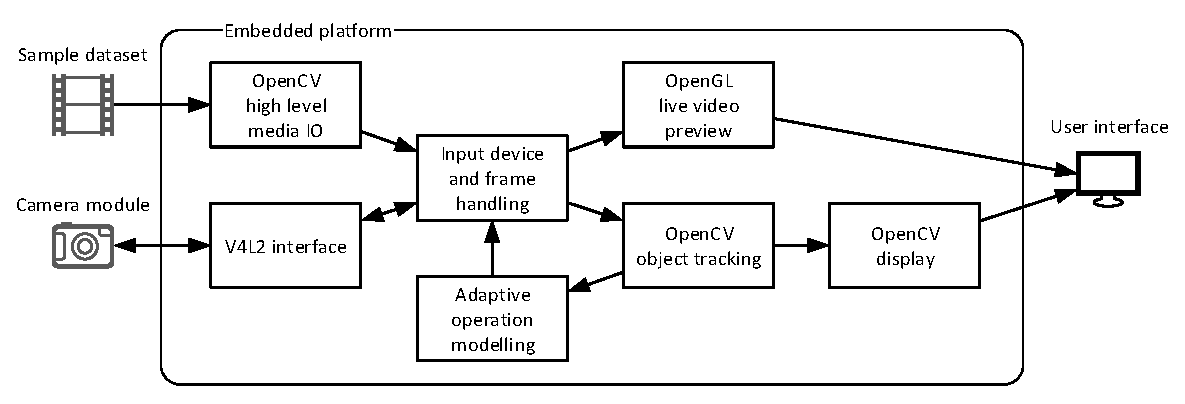
\includegraphics[width=\columnwidth]{block}
  \caption{Purposed system design block diagram.}
  \label{block}
\end{figure}

The entire system was based on an embedded platform. The application starts with reading video sequence from either a camera through V4L2 interface or sample datasets through OpenCV's media file IO APIs. It can also alter the camera frame interval, or skip video frames in the dataset. The frame read will be delivered to an independent OpenGL video preview thread for displaying on the screen. The frame will also be passed to object tracking algorithms that are based on OpenCV APIs. The algorithms will find moving objects, track them between frames, and render the results on the screen. The tracking results will also be used to predict an optimum frame rate. The desired frame rate will then be configured accordingly, hence the adaptive operation.
}

%{\color{red}Description required}

\section{Hardware}

% {\color{red}Design works, choices of hardware, software, etc.}

\subsection{Hardware platform}

%ARM or x86?

An embedded development board was used in this project, it enables easy power consumption analysis and \mdc{it} is more likely the situation where power efficiency will be required rather than a desktop or server environment.

The most broadly used and powerful embedded processor architecture is ARM. It has relatively high performance grade available, extensively hardware and software support including embedded Linux operating system with reasonable power consumption and \modc{various} power saving modes, therefore was chosen to be used in this project.

Specifically, the Jetson Tegra K1 embedded development platform \cite{NVIDIA:tk1} (\fref{des:board}) featuring a 2.32GHz quad-core ARM CPU and a CUDA enabled Tegra GPU, introduced by NVIDIA, was used in this project. It has a rich set of peripheral interfaces exported \mdc{enabling} low-level control and interfacing with a MIPI-CSI high resolution camera module and is powerful enough to develop programs and execute complex computer vision algorithms on board. The heterogeneous architecture with CUDA enabled GPU can also be fully utilised by the GPU module in the specifically optimised OpenCV library, \mdc{making} it particularly suitable for computer vision tasks.

\begin{figure}[htb]
  \centering
  \includegraphics[width=0.7\columnwidth]{board}
  \caption{The Jetson Tegra K1 embedded development board.}
  \label{des:board}
\end{figure}

There are other heterogeneous architecture embedded platforms with ARM CPU cores and ARM GPUs available, but ARM GPUs are currently not supported by OpenCV's GPU module, and the CPUs alone are probably not powerful enough for complex computer vision tasks.

% {\color{red}More}

A general x86 architecture computer running Microsoft Windows operation system with a webcam was also used for algorithm development and remote control of the embedded development board. Since most algorithm developments do not use platform specific features, they can be developed on a general computer then easily migrated to the embedded platform.

\subsection{Camera}

% Specific camera module to be used was not determined yet at the time this progress report was written, but it would be a high resolution camera module from OmniVision \cite{ovt} that can be easily interfaced and directly controlled with the peripheral interfaces on the Jetson TK1 platform. A Linux kernel module driver probably need to be developed in order to control the camera parameters and operations from program running in user space.

The Raspberry Pi camera module (\fref{des:cam}) was used in this project, it features a 5 mega pixels OV5647 camera sensor manufactured by OmniVision Technologies Inc. It is relatively more expensive than buying \mdc{a camera sensor alone}, but the raspberry pi camera module is more broadly available in small quantities and can be easily connected to the board without the need to design a dedicated adapter PCB. It uses the MIPI-CSI interface which the board has native support for, the complete data sheet is also available around the Internet and it features subsampling, frame rate control, auto exposure and white balance functions etc. which are essential to adaptive operation.

\begin{figure}[htb]
  \centering
  \includegraphics[width=0.3\columnwidth]{rpi_camera_front}
  \includegraphics[width=0.3\columnwidth]{rpi_camera_back}
  \caption{The Raspberry Pi camera module.}
  \label{des:cam}
\end{figure}

The only difficulty is that the camera sensor can only output frames in raw Bayer pattern format \cite{bayer1976color}, as shown \mdc{in} \fref{bayer}. A typical colourful computer image consists of 3 primary colour channels per pixel, which are red, green and blue, i.e. RGB colour space. However, because of physical and manufacture \mdc{constraints}, most of camera sensors including the camera used in this project have only one intensity sensor per pixel with a specific colour filter, arranged in Bayer pattern format, therefore image processing algorithm \moda{needs} to be applied to convert or approximate the raw data to produce full colour images. Some of the camera sensors have \moda{built-in image processors} that \mdc{apply} the algorithm automatically, but the Raspberry Pi camera sensor used in this project doesn't have that functionality, therefore the algorithm \moda{needs} to be implemented by the application. But since the format can be efficiently converted using the GPU cores and CUDA, that is not a significant issue.

\begin{figure}[H]
  \centering
  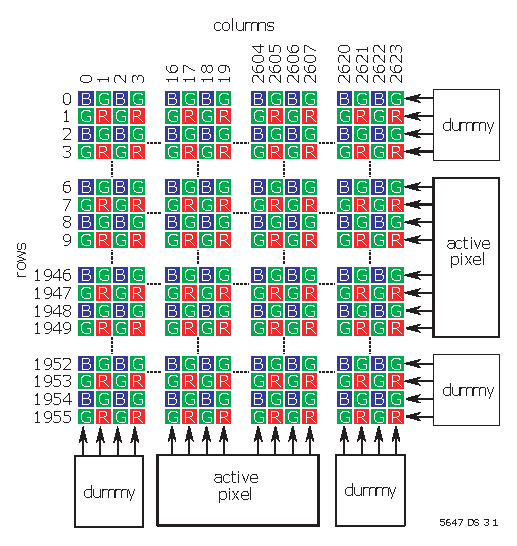
\includegraphics[width=0.6\columnwidth]{bayer}
  \caption{The Bayer pattern pixel arrangement used by the camera module (source from OV5647 datasheet).}
  \label{bayer}
\end{figure}

\section{Software}

\subsection{Operating system}

Ubuntu Linux distribution version 14.04.1 LTS was used on the platform \mdc{and} installed directly from the file system image provided by NVIDIA. Linux is great for this project because it is fully configurable, operating system overheads can be reduced to minimum by disabling unused services, even the graphical desktop environment. Also most Linux operations can be done through just command line interface, possibly via a SSH shell access, therefore programming and controlling the platform can be done anywhere with internet connection, which is very convenient.

The open-source GNU/Linux system also provides familiar and widely used tool sets, kernel driver development is well-documented, cross platform computer vision libraries especially OpenCV \mdc{are} also available \mdc{with} enormous community support.

\subsection{Computer vision API}

OpenCV \cite{opencv} was used to implement the algorithms, due to its cross platform adaptability, \modc{easy development} and large number of efficient algorithms ready for use and analysis. Furthermore, the OpenCV library for Jetson platform provided by NVIDIA had been further optimised, \mdc{providing} 2x-5x speed up \mdc{compared} to regular OpenCV \cite{NVIDIA:perf}. The OpenCV GPU module based on NVIDIA CUDA was also available\mdc{. It} utilises the heterogeneous architecture and provides 5x-20x speed up. These optimisations can reduce computation time dramatically, thus further \mdc{reduce} the power consumption.

\subsection{Testing dataset}

Using a consistent video stream input and a camera power consumption model instead of replaying the same scene in front of the camera is preferred, because reproducing the exactly same video stream from replaying scene is impossible\mdc{. Factors} such as camera and object instability, inaccurate synchronisation, hardware and software restrains will also take effect.

The \modc{CDNET video database} \cite{goyette2012changedetection} was used for testing the algorithms and analysing the performance and accuracy of adaptive operation. The database was rigorous and comprehensive\mdc{. It} involves lots of carefully chosen video streams from different real life scenarios, \mdc{and is} very useful for evaluate object tracking algorithms in different \mdc{situations}.

\section{Algorithms}

\subsection{Object detection algorithm}

The model based object detection algorithms described in previous chapter might be useful for some specific projects, but for a more general object tracking system with previously specified application areas, \moda{motion-based background subtraction} algorithms which can track any kind of moving objects, was used in this project for evaluating adaptive operation.

\moda{Other than background subtraction algorithm, there is another motion-based object detection algorithm described previously, the optical flow algorithm. However, there is a major limitation with it. Since optical flow can only detect moving objects, objects that are moving in a relatively low speed or stops for a few moments, would be undetectable by optical flow, and this scenario is very commonly found.} Therefore background subtraction that can handle this kind of situations was used for the object detection phase.

However, there are several distinctive background subtraction algorithms available for use. After some evaluations, the ViBe algorithm was chosen, because it is relatively efficient, with moderate memory usage and has \moda{GPU implementation that can take the advantages} of heterogeneous platform architecture.

\subsection{Object tracking algorithm}

Connected component analysis is used after foreground masks being extracted from each frame. Specifically, the simple \moda{"find contours"} function that is also used by the simple blob detector from OpenCV was used. It is very simple, but still sufficient to extract blobs from black and white masks without intensive computation.

%Afterwards, the good features to track function is used to determine feature points inside foreground masks, then related to the objects detected respectively.

\moda{Afterwards, the corner points of blobs extracted from foreground masks were used as feature points. Next,} sparse set optical flow will be applied to track the movements of feature points in following frames. By relating the feature points back to \moda{object blobs}, the objects can then be tracked.

% {\color{red}HOW???}

\chapter{Implementation}

\section{Camera driver}

The camera driver was implemented based on Linux Video for Linux second version (V4L2) framework. It is a great framework that supports varies kinds of different camera sensor models with the same user space interface, across vast number of different embedded Linux platforms, enables cross platform adaptability with accessibility to low level controls.

For adaptive operation, the driver implemented supports different resolution modes from the camera and changing frame interval in great precision. A special control instruction that can change any of the control registers inside the camera sensor was also developed for debugging and controlling purpose.

A GPIO connected to a LED on the camera module was also controllable through the driver, to give indications about camera activity, used for debugging purpose and triggering external power analyser.

\section{Application}

% {\color{red}Application structure, multithreading}
% Bayer pattern handling.
% Multi-threading:
% 	i. Camera thread for camera control, buffer swapping, synchronisation and management etc.
% 	ii. OpenGL preview thread shows the camera output in real time, can be suspended for power saving.
% 	iii. OpenCV worker thread running algorithms.
% 	iv. OpenCV viewing thread.
% 	Display results and handle GUI user input, slow, can be suspended for power saving.

\subsection{Bayer pattern handling}

A typical colourful computer image consists of 3 primary colour channels {\color{red}CITE}, which are red, green and blue. However, because of physical and manufacture constrains, most of camera sensors including the camera used in this project have only one intensity sensor per pixel of a specific colour, arranged in a special pattern called Bayer pattern {\color{red}CITE}, therefore image processing algorithm need to be applied to convert or approximate the raw data to produce full colour images. Some of the camera sensors have a built-in image processor that applies the algorithm automatically, but the camera used in this project doesn't have that functionality, therefore the algorithm need to be implemented by the application.

{\color{red}Some diagrams show how it is done.}

\subsection{Application structure}

An application was developed to receive video stream from the camera or read continuous frame images from the dataset, then apply OpenCV processing, real-time input and output video preview as well as camera control. To take the benefits of the heterogeneous architecture more efficiently and overcome issues with buffer updates, the application was implemented using a multi-threading approach with inter-thread synchronisation mechanisms.

The main thread is responsible for initialisation, camera control, capture buffer synchronisation and management. It allocates several buffers for the camera driver, assign filled buffers to other processing threads and recycle processed buffers back to camera driver.

Afterwards, an OpenGL video preview thread was used to show the frames captured from camera to a monitor, independent from algorithm processing. This thread can be independently stalled so that it would not consume any processing power when analysing performances and power consumptions of algorithms.

The OpenCV algorithms runs on both CPU and GPU, and OpenCV has a constrain that to view the processed images, the application needs to call a user interface update function that is time consuming but not power intensive, therefore 2 threads was used in a pipeline style in order to speed up the processing. The buffers received from main thread will first go through the processing thread, then pass to the second thread for display on the monitor. The display thread can also be stalled for power saving.

%The OpenCV algorithms runs on both CPU and GPU, therefore to take the full advantages of heterogeneous architecture and run the algorithms as fast as possible, the OpenCV processing runs in a pipelined style through 3 threads. Every buffer received will go through first CPU processing thread, then transferred to GPU processing thread, finally .
%and OpenCV has a constrain that to view the processed image results, the application, so that two OpenCV processing threads was created so that.

Finally, an input handing thread for debugging and controlling through command line interface. Most of time this thread is block waiting for user input, therefore won't consume considerable CPU time.

\section{Object detection algorithms}

\subsection{Colour based}

An simple implementation \cite{MOTBOC.git} of colour filtering object detection algorithm was investigated, as shown in \fref{Figure:MOTBOC}.

{\color{red}UPDATE!}
\begin{figure}[H]
  \centering
  \includegraphics[width=0.6\columnwidth]{"MOTBOC failure"}
  \caption{Simple multi object tracking based on colour \cite{MOTBOC.git} in ideal situation}
  \label{Figure:MOTBOC_F}
\end{figure}

However, this implementation is very limited, it can only detects objects with single colour, cannot distinguish the objects from similar background colour, relies heavily on manually adjusted colour threshold values, and is very sensitive to the variations of colour spaces from different cameras, therefore not very adaptable. A complex environment may also results into lots of undesired detections, as shown in \fref{Figure:MOTBOC_F}.

\begin{figure}[H]
  \centering
  \includegraphics[width=0.6\columnwidth]{"MOTBOC failure"}
  \caption{Simple multi object tracking based on colour \cite{MOTBOC.git} at a complex environment}
  \label{Figure:MOTBOC_F}
\end{figure}

{\color{red}Descriptions about the failure}

\subsection{Shape based}

OpenCV's implementation of Hough Circle Transform for circle detection was investigated, as shown by \fref{Figure:circles}.

%\fref{Figure:circles} shows the image processed by circle detection, based on OpenCV's implementation of Hough Circle Transform \cite{opencv:hough_circle}.

\begin{figure}[H]
  \centering
  \subfigure [] {
    \includegraphics[width=0.45\columnwidth]{simple_original}
    \label{Figure:edges:original}
  }
  \subfigure [] {
    \includegraphics[width=0.45\columnwidth]{simple_blur}
    \label{Figure:edges:blur}
  }
  \subfigure [] {
    \includegraphics[width=0.45\columnwidth]{simple_edges}
    \label{Figure:edges:edges}
  }
  \subfigure [] {
    \includegraphics[width=0.45\columnwidth]{simple_circles}
    \label{Figure:edges:circles}
  }
  \caption{Circle detection. \subref{Figure:edges:original} The original image, \subref{Figure:edges:blur} image converted to gray scale and blurred, \subref{Figure:edges:edges} edges detected, \subref{Figure:edges:circles} circles detected}
  \label{Figure:circles}
\end{figure}

The frame captured from camera (\fref{Figure:edges:original}), was first converted to a grey scaled and blurred image, as shown in \fref{Figure:edges:blur}. Blur or smoothing is often necessarily to reduce false object edges that might be detected. Afterwards the object edges in the image was extracted as in \fref{Figure:edges:edges}. Finally \fref{Figure:edges:circles} shows the circles detected by the algorithm.

However, this algorithm is still very limited and inaccurate, as shown by \fref{Figure:circles}, the coin at the top right corner had not been detected, because it appeared to be an eclipse instead of a prefect circle to the algorithm because of camera perspective. Furthermore, in order to detect multiple geometric shapes, different algorithms would be required for each of the different shapes.

\subsection{Cascade Classifier}

% as shown in \fref{Figure:cc_face}

The OpenCV's cascade classifier implementation \cite{opencv:cc} of face and eye detection was investigated as shown in \fref{Figure:cc_face}.

\begin{figure}[H]
  \centering
  \includegraphics[width=0.6\columnwidth]{"CC face"}
  \caption{Face and eye detection cascade classifiers, detected face was circled by pink, whereas detected eyes were circled by blue}
  \label{Figure:cc_face}
\end{figure}

Noticeable {\color{red}DATA?} frame rate drop and latency was experienced (about only {\color{red}xx} fps) when experiments with the cascade classifier implementation on the testing platform, suggests it might not be a suitable algorithm for real-time object tracking application. In addition, multiple classifier definition files were required for detecting different kinds of objects, or even different perspectives of the same object, which would require lots of computations.

\subsection{Motion based}

The article \cite{bgs:article} reviewed the algorithms available in the BGSLibrary, ranked 5 algorithms as the best methods for accuracy. Except the Pixel-Based Adaptive Segmenter (PBAS) algorithm which was removed due to patent issues, the other 4 algorithms listed in \tref{Table:bgs} were investigated in this project.

\begin{table}[H]
  \centering
  \begin{tabular}{cc}
  \toprule
  \textbf{Method ID} & \textbf{Method name}\\
  \midrule
  MultiLayerBGS & Multi-Layer BGS \\
  MixtureOfGaussianV1BGS & Gaussian Mixture Model \\
  LBAdaptiveSOM & Adaptive SOM \\
  DPWrenGABGS & Gaussian Average \\
  \bottomrule
  \end{tabular}
  \caption{Background substraction algorithms investigated (adapted from \cite{bgslibrary})}
  \label{Table:bgs}
\end{table}

\fref{Figure:bgs_frame} shows the foreground masks obtained from those 4 algorithms through 2 sample frame sequences available with the BGSLibrary \cite{bgslibrary}.

\begin{figure}[H]
  \centering
  \includegraphics[width=0.24\columnwidth]{bgs_frame/MultiLayerBGS/input}
  \includegraphics[width=0.24\columnwidth]{bgs_frame/MultiLayerBGS/mask}
  %\includegraphics[width=0.32\columnwidth]{bgs_frame/MultiLayerBGS/bkgmodel}
  \includegraphics[width=0.24\columnwidth]{bgs_video/MultiLayerBGS/input}
  \includegraphics[width=0.24\columnwidth]{bgs_video/MultiLayerBGS/mask}

  \includegraphics[width=0.24\columnwidth]{bgs_frame/MixtureOfGaussianV1BGS/input}
  \includegraphics[width=0.24\columnwidth]{bgs_frame/MixtureOfGaussianV1BGS/mask}
  \includegraphics[width=0.24\columnwidth]{bgs_video/MixtureOfGaussianV1BGS/input}
  \includegraphics[width=0.24\columnwidth]{bgs_video/MixtureOfGaussianV1BGS/mask}
  %\includegraphics[width=0.32\columnwidth]{na}

  \includegraphics[width=0.24\columnwidth]{bgs_frame/LBAdaptiveSOM/input}
  \includegraphics[width=0.24\columnwidth]{bgs_frame/LBAdaptiveSOM/mask}
  \includegraphics[width=0.24\columnwidth]{bgs_video/LBAdaptiveSOM/input}
  \includegraphics[width=0.24\columnwidth]{bgs_video/LBAdaptiveSOM/mask}
  %\includegraphics[width=0.32\columnwidth]{na}

  \includegraphics[width=0.24\columnwidth]{bgs_frame/DPWrenGABGS/input}
  \includegraphics[width=0.24\columnwidth]{bgs_frame/DPWrenGABGS/mask}
  \includegraphics[width=0.24\columnwidth]{bgs_video/DPWrenGABGS/input}
  \includegraphics[width=0.24\columnwidth]{bgs_video/DPWrenGABGS/mask}
  %\includegraphics[width=0.32\columnwidth]{na}
  \caption{Results obtained from background subtraction algorithms. From left to right column: input sample 1, foreground mask obtained, input sample 2, foreground mask obtained. From top to bottom row: MultiLayerBGS, MixtureOfGaussianV1BGS, LBAdaptiveSOM and DPWrenGABGS.}
  \label{Figure:bgs_frame}
\end{figure}

It can be seen from \fref{Figure:bgs_frame} that MultiLayerBGS gave the best foreground masks, but it was also the slowest algorithm on the testing platform.

\section{Object tracking algorithms}

Connected component analysis or blob detection (\sref{blob}) and movement tracking (\sref{bg:tracking}) algorithms were not implemented yet.

A suitable camera module need to be ordered and interfaced afterwards, then implement automatic feedback control of frame rate, cropping and down sampling.

\section{Adaptive power saving}

\section{Video stream dataset}

\chapter{Analysis} \label{Chapter:Analysis}

\section{Camera frame rate}
\label{ana:cam:fps}

The camera frame rate was calculated as shown by \eref{ana:cam:eq:rate}. The number of lines in a frame can be easily changed by adding dummy lines after the actual frame data. The time required for transmitting synchronisation packet is negligible, thus there are no extra constants in the equation.

\begin{equation}
	f = \frac{\text{Number of lines in a frame data}}{\text{Transmission time of 1 line of data}}
	\label{ana:cam:eq:rate}
\end{equation}

To verify the equation, the transmission times of an entire frame and individual lines were measured using an oscilloscope as shown in \fref{ana:cam:osc:time}. From the cursor measurements shown in the oscilloscope screen captures, the transmission time of an frame is $10.21917 ms$ and $206.45 \mu s$ for 10 lines. It matches the equation precisely. The camera frame rate conversion function in the application was constructed according to these figures.

\begin{figure}[!htb]
  \centering
  \subfigure [Measuring frame interval from synchronisation packets] {
    \includegraphics[width=0.9\columnwidth]{camera/osc/frame}
  }
  \subfigure [Measuring transmission time of 10 lines] {
    \includegraphics[width=0.9\columnwidth]{camera/osc/line}
  }
  \caption{Measuring the transmission time of an entire frame and individual lines.}
  \label{ana:cam:osc:time}
\end{figure}

However, when experimenting with changing frame rate, a software constraint was discovered. The MIPI-CSI driver developed by NVIDIA can only effectively handle frame rates equal or higher than 5 FPS. For frame rates less than 5 FPS, the camera still functioning as expected, but the driver will be desynchronised. Almost half of frames transmitted from the camera will be lost. As a result, the adaptive operation should not run below 5 FPS.

Another important constraint is the frame rate cannot be changed drastically. When changing the frame interval, camera sensor exposure time, gain control and white balance need to be adjusted at the same time. This is handled by the automatic exposure, gain and white balance adjustment functions on the image sensor processor (ISP) inside camera sensor. The automatic adjustments were implemented with a feedback loop approach. Consequently, when changing the frame interval drastically, the adjustments needed are also significant. As a result, the first few frames captured after such a change will be significantly different from previous frames in brightness and white balance. That is enough to confuse the object tracking algorithms. A software limitation of frame interval changing rate was therefore added in the application. This may be resolved by using software compensation algorithm, but it will required lots of investigations, not possible at this time.

%\todo{BOOM}

\todo{Oscilloscope waveform of frame rate changing.}

\section{\todo{Object tracking algorithms}}

\section{Power consumption modelling}

To measure power consumption, 10 resistors of $10 \Omega$ were connected in parallel to gives a precise $1 \Omega$ resistance and allows high current flow through. Then the resistors was connected in series with the board power supply as shown in \fref{ana:power:sch}. The fan used for CPU cooling can be replaced by passive cooling systems in actual application, thus was powered from an external power source instead of the board during power consumption analysis.

\begin{figure}[H]
  \centering
  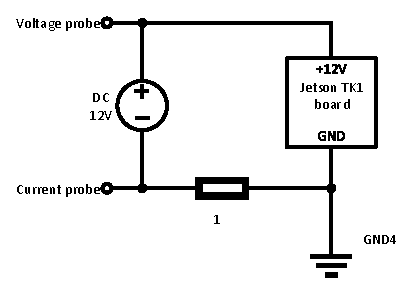
\includegraphics[width=0.6\columnwidth]{ana_power_sch}
  \caption{Schematic of measuring power consumption using oscilloscope.}
  \label{ana:power:sch}
\end{figure}

The average power consumptions of the complete system running the object tracking algorithms at different frame rates were measured as shown in \fref{ana:cam:osc:power}. The current probe was set according to the $1 \Omega$ series resistance, gives accurate current waveform. Maths function on the oscilloscope was used to multiply voltage and current waveforms together, produces power waveform in real-time. The oscilloscope was then set to record 20 million samples of the waveforms in a period of 10 seconds, averaged together to give the average power rating over the period.

\begin{figure}[htb]
  \centering
  \includegraphics[width=0.9\columnwidth]{camera/osc/power}
  \caption{Screen capture of measuring power consumption using oscilloscope.}
  \label{ana:cam:osc:power}
\end{figure}

Multiple measurements were attempted, then averaged to give the final results shown in \fref{ana:cam:power}. The frame rates chosen were focused on the discrete frame rates used during datasets evaluation.

\begin{figure}[htb]
  \centering
  \subfigure [Detailed data from power consumption measurements] {
    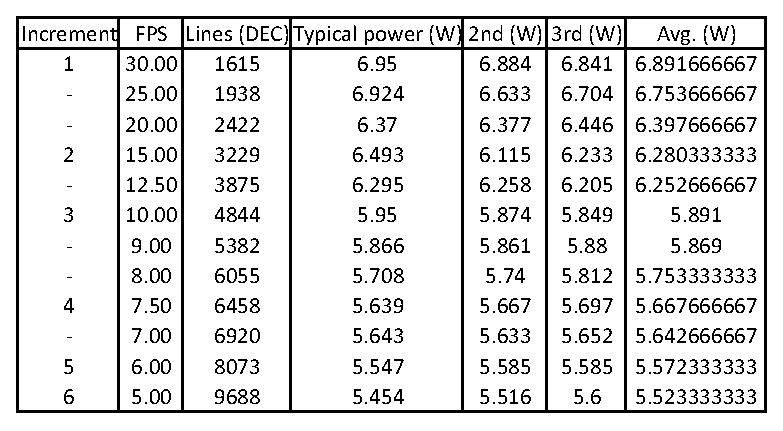
\includegraphics[width=0.55\columnwidth]{ana_cam_data}
  }
  \subfigure [Power consumption ploted against frame rate] {
    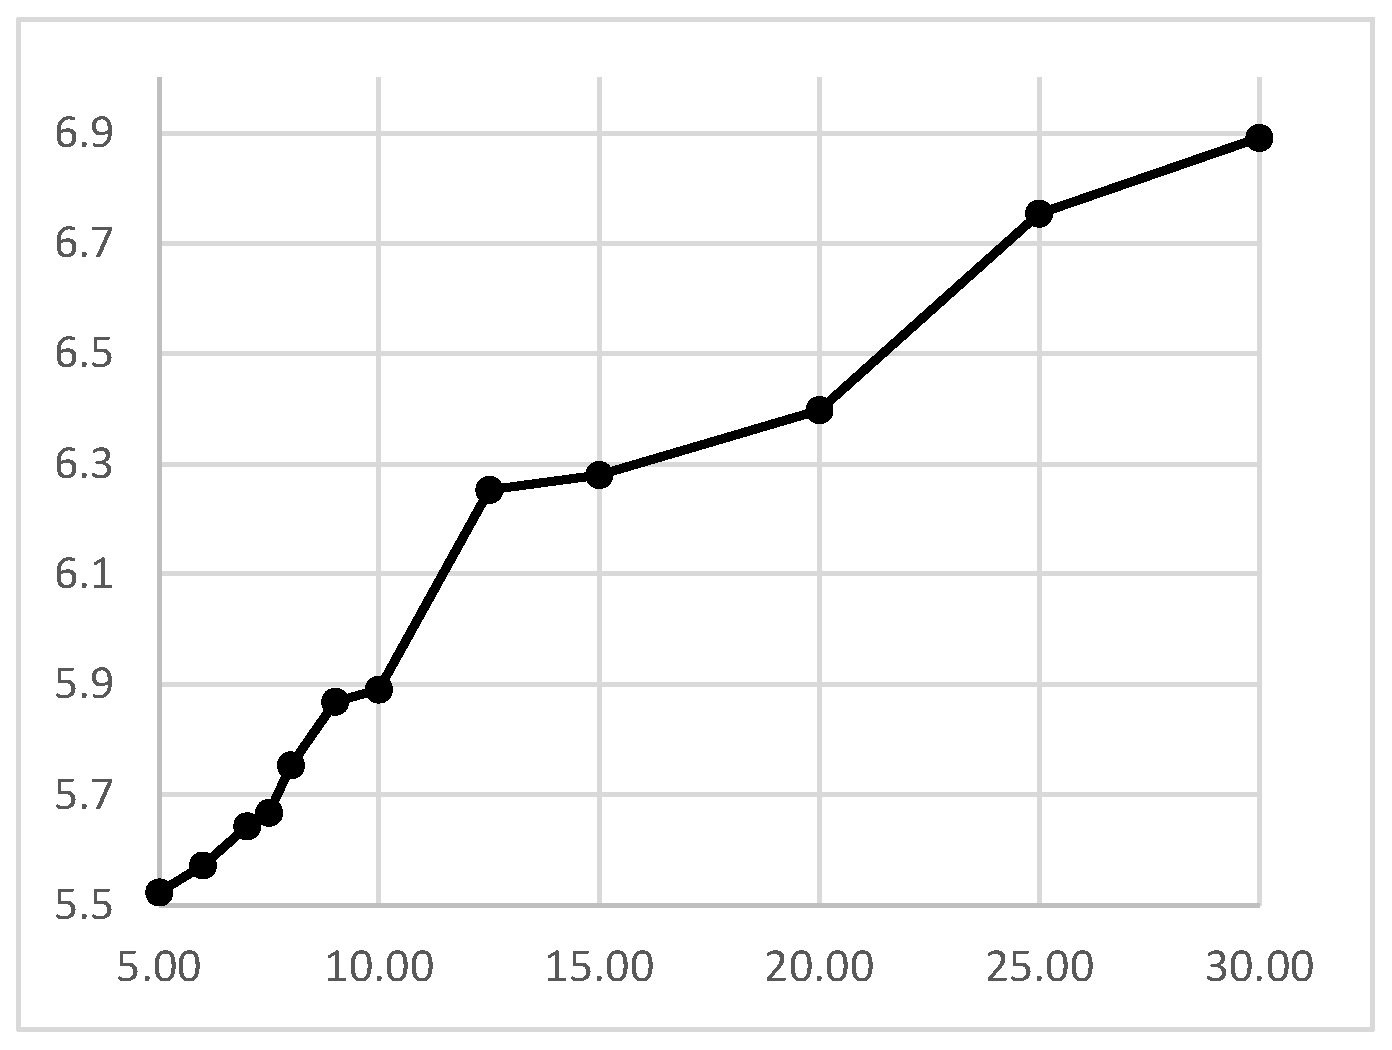
\includegraphics[width=0.35\columnwidth]{ana_cam_chart}
  }
  \centering
  \caption{Power consumptions measured against different frame rates.}
  \label{ana:cam:power}
\end{figure}

%\todo{BOOM}

\section{Power consumption reduction analysis}

Power consumption reduction was analysed using the video datasets from CDNET, to keep input video stream consistent. However, due to the frame images inside the datasets are discrete in time, the frame rate cannot be changed in great precision. The results obtained will only be a rough estimation of the actual performance in actual application.

Some properties of the dataset under test need to be determined first, such as maximum object moving speed and minimum FPS required. This is done by evaluate the dataset without adaptive operation. During the process, the maximum distances objects moved between each frame intervals were recorded. The top $5 \%$ of the distances that are most likely due to errors were removed. \fref{ana:ada} shows the distribution of maximum moving distances after filtering in a dataset. The maximum of those value was considered as the maximum speed an object may travel in the dataset. According to the formulae described in section \ref{imp:ada:metric}, the minimum FPS requirement was then calculated. The optical flow tracking window was set to 32 pixels, as a result most minimum FPS requirements calculated were under 1 FPS. However, to match the constraints of the camera driver as described in section \ref{ana:cam:fps}, the minimum FPS was set to 5 FPS.

\begin{figure}[htb]
  \centering
  \subfigure [Absolute maximum distances objects travelled between frames] {
    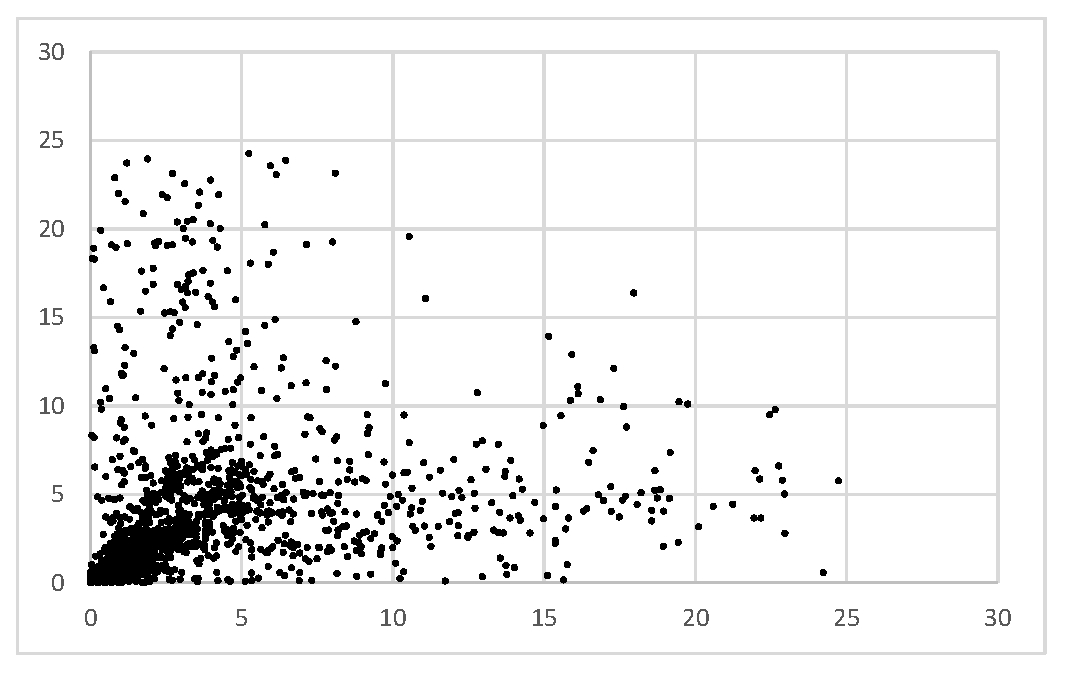
\includegraphics[width=0.45\columnwidth]{ana_ada_xy}
    \label{ana:ada:xy}
  }
  \subfigure [Histogram distribution of maximum distances] {
    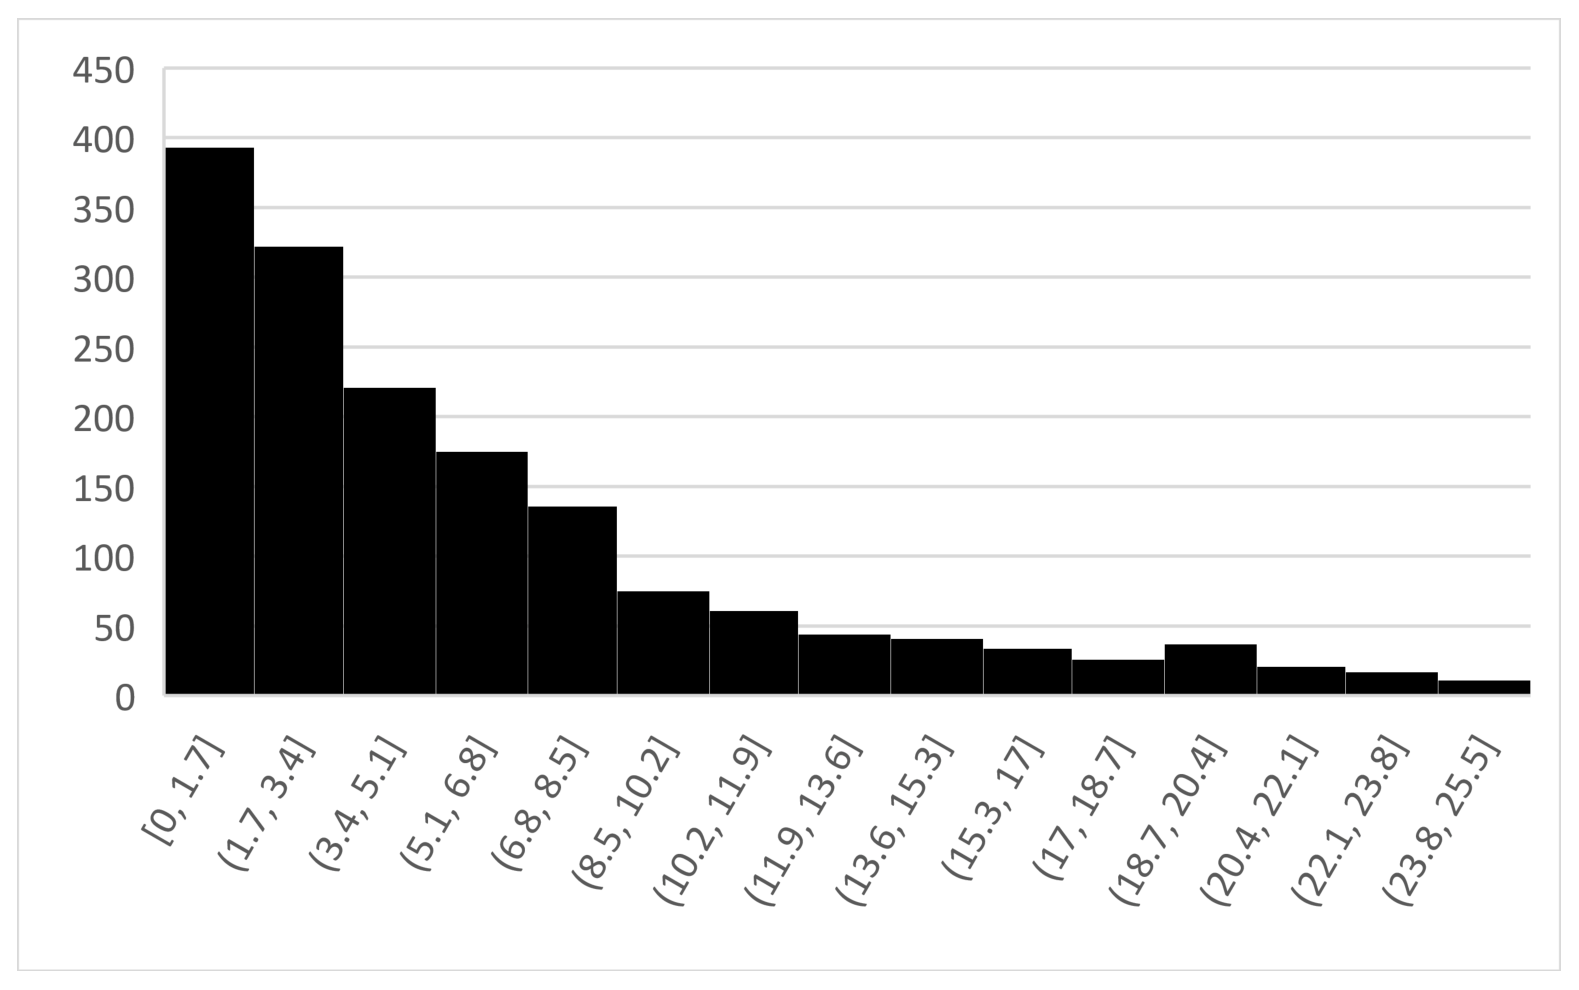
\includegraphics[width=0.45\columnwidth]{ana_ada_histo}
    \label{ana:ada:histo}
  }
  \caption{Filtered distributions from CDNET highway dataset.}
  \label{ana:ada}
\end{figure}

Moving blobs that are continuously connected by the tracking algorithm across frames were considered as being tracked. The speed of objects moving in the datasets are relatively low to the frame rate, all the objects in the datasets evaluated are considered as being tracked regardless of adaptive operation.

By applying the power consumption model, the power consumption reduction can be estimated, summarised in \fref{ana:summary}.

\begin{figure}[htb]
  \centering
  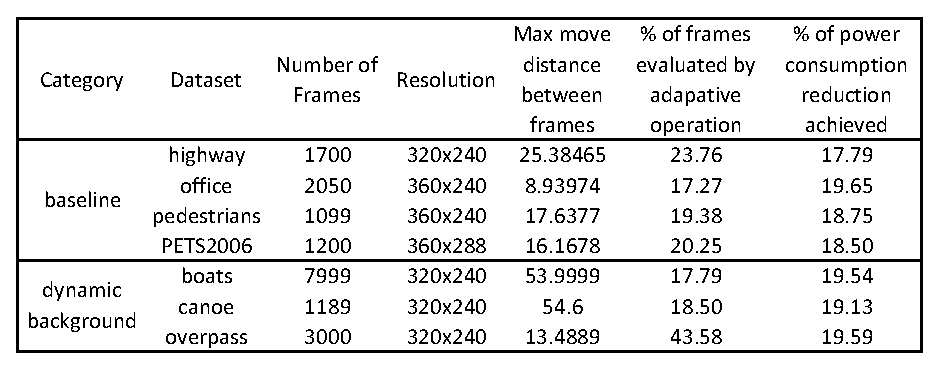
\includegraphics[width=\columnwidth]{ana_summary}
  \caption{Summary of results from evaluated CDNET datasets.}
  \label{ana:summary}
\end{figure}

\chapter{Conclusion} \label{Chapter:Conclusion}

\section{Achievements}

The camera driver was successfully developed, and was able to configure the camera sensor, capture still images and video streams.

Several object detection and tracking algorithms were investigated.

An application running adaptive object tracking algorithms was developed. The algorithms can run at 30 FPS as in specification. The effect of adaptive operation was investigated. All objects in the sample datasets get tracked regardless of whether the adaptive operation is applied or not.

By applying adaptive operation, power consumption reduction estimation of $19 \%$ was achieved for varies video surveillance datasets. It was only $19 \%$, due to the high standby power consumption of the embedded development board. The adaptive operation still has an effect on power consumption, but was not very significant compare to standby power consumption.

%\todo{Power saving achieved.
%Compare back to aims, specifications. (Why didn't?)}

\section{Constraints}

The algorithms used can only run at around 30 FPS maximum with $320 \times 240$ resolution. Objects moves faster than this, such as a basket ball may need a faster frame rate to be tracked. The maximum speed is also highly depending on the object to camera distance.

The algorithms implemented can only works with a steady background, limiting the application area to still camera application such as video surveillance.

\section{Further work}

\subsection{Camera driver}

The camera driver in collaboration with NVIDIA's MIPI-CSI driver is not stable enough. In case the application that are using the camera being forced stopped by the user or due to a programming bug, the drivers may crash the kernel due to lost synchronisation. This need further investigation.

When a buffer been marked as filled by the MIPI-CSI driver, it is actually still receiving data from the camera. Possible reasons are losing or misinterpreting synchronisation packets, camera configuration problem and bugs in MIPI-CSI driver implementation. A workaround was used, by receiving 2 filled buffers from the driver, then use the first one as valid data. However, this workaround gives 2 frames latency regardless of frame rate. This need further investigation.

The driver interface for controlling the frame rate, configuring exposure settings etc. need to be completed and standardised.

The Tegra K1 CPU has a built-in ISP that can convert Bayer pattern to standard RGB format without using CPU or GPU time. However, the documentation of this feature is confidential. The NVIDIA's video interface driver that are using this ISP is also undocumented in public domain. Power consumption may be reduced further if the ISP can be used.

\subsection{Application}

The application structure may be made more efficient.

The application can be a lot easier to use and configure with a better user interface.

Transmission of video stream and tracking results through network for Internet-of-Things applications may be useful to implement.

\subsection{Algorithms}

Further optimisations to the algorithms are possible. More efficient implementations that supports better resolution and faster frame rate are desired.

Blob tracking algorithm based on optical flow tracking results may be implemented.

More algorithms may be investigated. Especially algorithms that handle background movement, which are very useful in automotive applications.

\section{Evaluation}

During implementation, I found that I spent a lot time trying to stabilise the camera driver to prefect. That is not the main goal of the project, the camera driver was actually usable for algorithm analysis. Therefore I chose to accept the problems with the drivers, and moved the diagnosis works to further work.

%\todo{Difficulties, solutions etc.}

\chapter{Project management}

\section{Risk assessment}

\section{Time management}

The topic of project changed once during week 7 in semester 1. The previous topic (\aref{Appendix:brief_prev}) was about reducing power consumption for algorithms that are utilising General Purpose GPU (GPGPU) technique, by adaptively controlling calculation precision. The NVIDIA Jetson TK1 development platform was decided to be used in this project. However, after investigated into the topic and experimented with some algorithms, the purposed precision control did not contribute significant impact on computation quality. Not much power saving would be possible to be made.

Therefore, I decided to change the project topic. The current project topic (\aref{Appendix:brief}) was quickly determined. The same hardware platform was still used, so that the time invested in the previous project was not wasted. Therefore, I was able to quickly catch up with the progress.

The Gantt chart was also changed due to project topic changing, as shown in \aref{Appendix:gantt}. The time invested for previous project topic was treated as background reading.
\todo{GANTT CHART UPDATE}

\section{Backing up}

%Source code management.
%Documents and materials.

The git version control system \cite{git} was used in this project. It has the feature that allows multiple users collaborate on the same repository. However, this is an individual project, git was used purely for backing up source code version history and synchronisation between multiple devices. Well-known git hosting website GitHub \cite{github} and university's SourceKettle server \cite{sourcekettle} were used for multiple backups.

All documents, background literals and materials used by the project were backed up using Microsoft's OneDrive service.

%\section{Remaining work}

%\begin{itemize}
%  \item Movement tracking based on blob detection (Section \ref{bg:tracking}, \ref{impl:tracking}).
%  \item A camera module need to be ordered and interfaced.
%  \item Automatic frame rate reduction based on tracking result.
%  \item Hardware downsampling and cropping based on ROI.
%  \item If time allows, energy-efficient object recognition may be implemented.
%\end{itemize}


%\appendix

\titleformat{\chapter}[hang]{\Large\bfseries}{\chaptertitlename\ \thechapter}{0.75cm}{\Large\bfseries}
\begin{appendices}
%% ----------------------------------------------------------------
%% Appendix:brief
%% ----------------------------------------------------------------
\chapter{Agreed project brief}
\label{Appendix:brief}

\begin{figure}
\centering
\includepdf[pages={1}, offset=0 -2cm, trim={0, 0, 0, 0}, clip]{inc/Brief.pdf}
\end{figure}

\clearpage

%% ----------------------------------------------------------------
%% Appendix:brief_prev
%% ----------------------------------------------------------------
\chapter{Previous project brief}
\label{Appendix:brief_prev}

\begin{figure}
\centering
\includepdf[pages={1}, offset=0 -2cm, trim={0, 0, 0, 0}, clip]{inc/Brief_previous.pdf}
\end{figure}

\clearpage

%%% ----------------------------------------------------------------
%% Appendix:gantt
%% ----------------------------------------------------------------
\chapter{Project Gantt charts}
\label{Appendix:gantt}

\begin{figure}[H]
  \centering
  \subfigure [{Previous Gantt chart}] {
    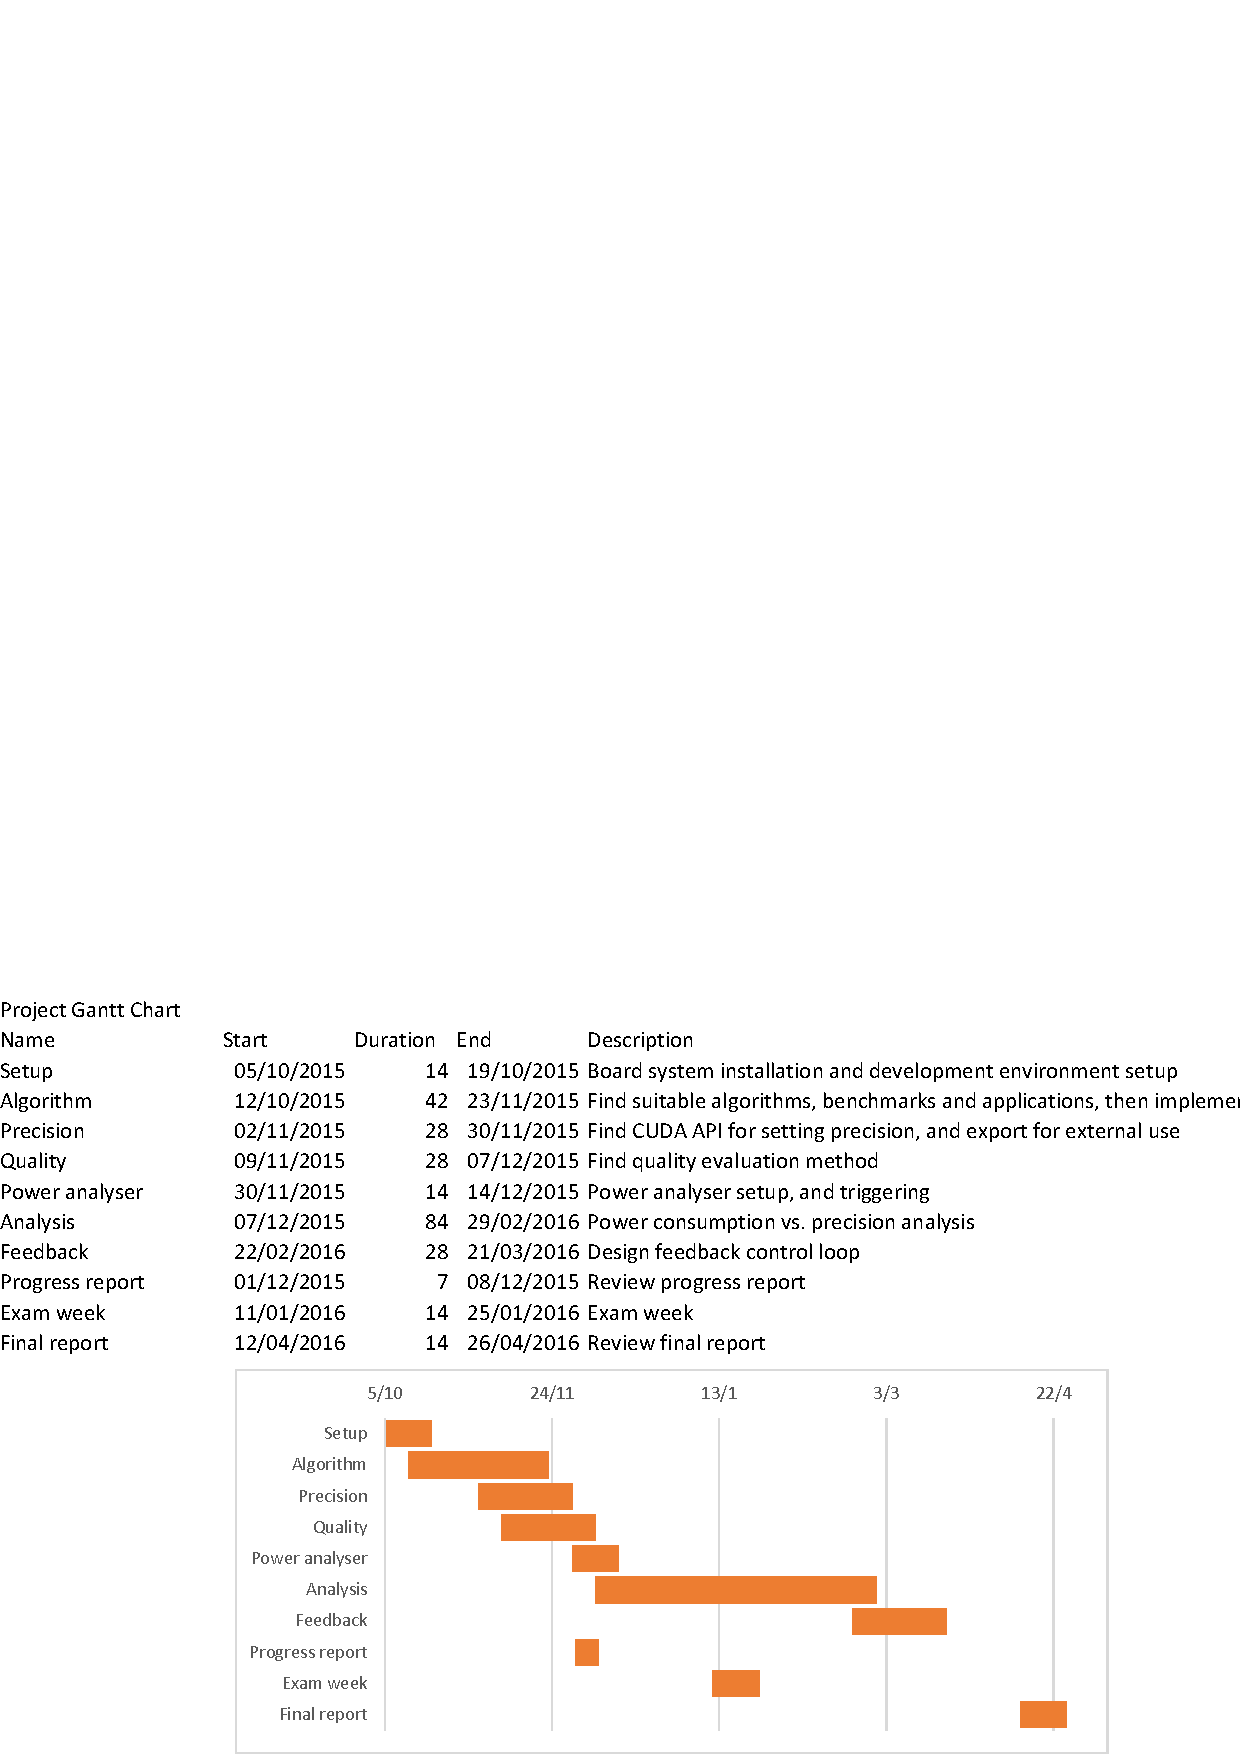
\includegraphics[page=1, trim={1cm, 5cm, 4cm, 1cm}, clip, width=\columnwidth]{inc/Gantt_previous.pdf}
  }
  \subfigure [{Current Gantt chart}] {
    \includegraphics[page=1, trim={1cm, 5cm, 4cm, 1cm}, clip, width=\columnwidth]{inc/Gantt.pdf}
  }
\end{figure}

\clearpage

\chapter{Costs} \label{Appendix:Costs}

Bill of materials

\clearpage

\chapter{Contents of design archive} \label{Appendix:Archive}

\begin{table}[!htb]
  \centering
  \begin{tabular}{|l|l|}
  \hline
  \textbf{Path} & \textbf{Description} \\ \hline
  Bayer/ & CPU implementation of Bayer pattern conversion. \\ \hline
  bgslibrary/ & The BGSLibrary. \\ \hline
  Datasheet/ & Camera module datasheet and GPIO allocations. \\ \hline
  Images/ & Some useful images and screen captures.\\ \hline
  kernel/ & Camera driver and kernel source modifications. \\ \hline
  OpenCV/ & OpenCV algorithms implemented on a general computer. \\ \hline
  opencv2/ & Non-free ViBE GPU module. \\ \hline
  OpenCVTegra/ & OpenCV algorithms implemented on the Jetson board. \\ \hline
  %report/ & Source code of this report in LaTeX. \\ \hline
  scripts/ & Various Linux shell scripts for testing process. \\ \hline
  V4L2 & The adaptive object tracking with camera application. \\ \hline
  \end{tabular}
  \caption{Contents of design archive}
\end{table}

\clearpage

\end{appendices}

\backmatter
\bibliography{Reference}

\end{document}
%% ----------------------------------------------------------------
